%===============================================================================
% sample.tex
% Sample structure for RW344 essays.
%===============================================================================

\documentclass[11pt,a4paper,twocolumn]{article}
\usepackage{a4wide}
\usepackage{graphicx}
\renewcommand{\baselinestretch}{1.1}
\setlength\overfullrule{5pt}

% -- DO NOT CHANGE THE SETTINGS ABOVE --

\begin{document}
\title{
	TCP Congestion Control Comparison
}
\author{
	Arne Esterhuizen
}
\date{20 Janaury 2012}
\maketitle

\begin{abstract}
The purpose of this report is to investigate the effects that different TCP variants have on each other.
These TCP variants differ by the congestion control algorithms they employ. Congestion control algorithms affect
how much network traffic is generated by TCP at any one time and aims to prevent a TCP connection from over utilising
the network. This report investigates the different congestion control algorithms that are included as loadable
modules in the Linux kernel, and discusses experiments performed on how these congestion control algorithms compete
for network resources. It will be shown that some TCP variants are able to co-exist, whilst others tend to 
use excessive bandwidth, potentially smothering other competing TCP connections.
Should the results prove interesting, the project may be given to third year computer network students to 
perform as an assignment.
\end{abstract}

\section{Table of Contents}

\section{Introduction}
\label{sec:intro}

The \textit{Transmission Control Protocol} (TCP) controls how much data it transmits over a network by utilising
a congestion window. TCP cannot send more data than the congestion window allows. The size of TCP's congestion
window depends on the condition of the network. In the case of the network experiencing heavy data traffic, the congestion window
would be shortened. In the case of the network being only lightly loaded with data traffic, the congestion window would
be expanded. How and when to adjust the congestion window depends on whatever form of congestion control
a TCP connection utilises. Congestion control algorithms rely on various indicators to passively ascertain the state of the network.
Packet loss is an indication that the network is being over utilised and that routers along the way are dropping IP packets
due to limited buffer space. Also, routers can set special flags in an IP packet's header that will inform the receiving host
that congestion is about to occur. The receiving host can then inform the the sending host to reduce its sending rate.
Other methods include closely observing packet round trip times as well as determining the queueing delay, the time packets
spend waiting in a router's buffer.
Using one or more of these methods, congestion control algorithms are able to adjust their behaviour according to whether congestion
has occurred or could occur. As will be seen, some congestion control mechanisms allow for unfair usage of network bandwidth,
while others are able to share bandwidth equally.

The different congestion control mechanisms available for use by the Linux kernel are:
\begin{itemize}
\item HTCP
\item Hybla
\item Illinois
\item LP
\item Vegas
\item Reno
\item BIC
\item Westwood
\item YeAH
\item Cubic
\item Highspeed
\item Scalable
\item Veno
\end{itemize}
The linux socket interface allows one to change the type of congestion control a TCP connection uses by setting
the appropriate socket option.

A short description of the congestion control algorithms is given in section \ref{sec:tcpoverview}. Experiments were
performed to see how these algorithms compete against each other for bandwidth. A description
of these experiments is given in section \ref{sec:exp}, followed by a discussion of the results in section \ref{sec:results}.
Technical difficulties that may affect the practicality of this project as an assignment for students is described
is section \ref{sec:diff}. Section \ref{sec:conc} summarises the presented results.

\section{Overview of TCP variants}
\label{sec:tcpoverview}

\section{Experiments performed}
\label{sec:exp}
Experiments were carried out using client and server programs. A host running a client program generates data which is sent over the
network to a host running the server program. A single server host receives data from various client hosts. Each client host is set to use a different congestion control algorithm.
The amount of data received from client hosts is measured in megabits per second and is presented as a graph. This shows how much bandwidth the client host is able to utilise.
The mean of a client's bandwidth measurements is used to determine it's bandwidth usage in general. In these experiments, the highest possible throughput on the
network is slightly over 100 Mbps.

The experiments were run on the Stellenbosch University network. All hosts involved were located on the same network segment. All experiments
were carried out in the same manner, and all TCP variants were tested in pairs. Host A (a client) transmits data to host B (the server), after which host C (another client) also commences
sending data to host B. Thus the two client hosts do not commence with data transmission simultaneously, there is always a short delay between
one client beginning its transmission and the next client beginning its transmission. Therefore, the first client to commence transmission
always utilises the network freely, and is only forced to share bandwidth as soon as an additional client commences transmission.
This was found to have an impact on the behaviour of certain TCP variants, as their bandwidth utilisation appeared to change depending
on the order in which they were allowed to start (refer to section \ref{subsec:illinois}).

Every TCP congestion control algorithm was tested against all other algorithms, including itself. This was done in order to establish whether TCP variants
could be placed into groups in which all members are well behaved. 

\section{Results}
\label{sec:results}

As mentioned in section \ref{sec:exp}, all TCP variants were compared to each other. The results of these experiments will
be discussed in this section for each TCP variant individually. To avoid filling up this report with over 120 images, only
the most interesting results will be illustrated by showing the graph produced by the experiment.

\subsection{HTCP}
TCP HTCP is able to co-exist with itself, with each HTCP client having a mean throughput of 52 Mbps. HTCP has the lower throughput against Illinois, BIC, Westwood, and Scalable. 
Against Illinois, BIC, and Scalable, HTCP has a mean throughput in the range of 38 to 41 Mbps. Against Westwood, HTCP
has a throughput of 19 Mbps. HTCP is stronger against Hybla, LP, Vegas, Reno, YeAH, Cubic, and Highspeed. Against these it maintains a mean throughput
in the range of 64 to 67 Mbps. The exception is vegas, against which HTCP has a mean throughput of about 95 Mbps.

\begin{table}[h!]
	\begin{center}
		\begin{tabular}{| c | c | l |}
    			\hline
			\multicolumn{3}{|c|}{Mean Throughput (Mbps)} \\
    			\hline
    			HTPC &  \multicolumn{2}{|c|}{Other}  \\
			\hline
    			52 & 52 & HTCP \\
			\hline
    			66 & 37 & Hybla \\
			\hline
    			38 & 65 & Illinois \\
			\hline
    			65 & 38 & LP \\
			\hline
    			95 & 10 & Vegas \\
			\hline
    			66 & 37 & Reno \\
			\hline
    			41 & 62 & BIC \\
			\hline
    			19 & 86 & Westwood \\
			\hline
    			64 & 40 & YeAH \\
			\hline
    			67 & 37 & Cubic \\
			\hline
    			64 & 40 & Highspeed \\
			\hline
    			41 & 64 & Scalable \\
    			\hline
    		\end{tabular}
  	\end{center}
  	\caption{Mean throughput of HTCP against other TCP variants.}
	\label{table:htcp}
\end{table}

\subsection{Hybla}
\label{subsec:hybla}
Referring to table \ref{table:hybla}, Hybla seems to be able to co-exist with itself, LP,
Reno, Cubic, and YeAH. Hybla seems to do badly against Illinois, BIC, Westwood, and Scalable.

\begin{table}[h!]
	\begin{center}
		\begin{tabular}{| c | c | l |}
    			\hline
			\multicolumn{3}{|c|}{Mean Throughput (Mbps)} \\
    			\hline
    			Hybla &  \multicolumn{2}{|c|}{Other}  \\
			\hline
    			37 & 66 & HTCP \\
			\hline
    			52 & 51 & Hybla \\
			\hline
    			33 & 70 & Illinois \\
			\hline
    			48 & 54 & LP \\
			\hline
    			94 & 10 & Vegas \\
			\hline
    			49 & 54 & Reno \\
			\hline
    			28 & 75 & BIC \\
			\hline
    			14 & 90 & Westwood \\
			\hline
    			46 & 57 & YeAH \\
			\hline
    			53 & 50 & Cubic \\
			\hline
    			40 & 63 & Highspeed \\
			\hline
    			29 & 74 & Scalable \\
    			\hline
    		\end{tabular}
  	\end{center}
  	\caption{Mean throughput of Hybla against other TCP variants.}
	\label{table:hybla}
\end{table}

\subsection{Illinois}
\label{subsec:illinois}
As can be seen from table \ref{table:illinois}, Illinois is a very unfriendly, and
is unable to fairly share bandwidth with any other congestion control algorithm. The only congestion control algorithm to maintain a higher mean throughput than Illinois is Westwood. Illinois has the curious trait
of not being able to co-exist with even itself, something all of the other congestion control algorithms are
capable of.

In section \ref{sec:exp} it was mentioned that in some cases the order in which clients are allowed to begin transmission influences the bandwidth utilised. Illinois is one algorithm for which this applies. In table
\ref{table:illinois}, Illinois is allowed to begin transmission first, and even after a second client begins
transmitting data, Illinois still maintains a very high mean throughput. However if the order of transmission
is reversed, the competing client is allowed much more bandwidth, even if it is still less than Illinois.
This is illustrated by figures \ref{fig:illinois_yeah} and \ref{fig:yeah_illinois}. Illinois shows similar
behaviour with all other TCP variants, with the exception of Westwood and Vegas, whose mean
throughput remains the same ragardles of the order in which they start transmitting.

\begin{table}[h!]
	\begin{center}
		\begin{tabular}{| c | c | l |}
    			\hline
			\multicolumn{3}{|c|}{Mean Throughput (Mbps)} \\
    			\hline
    			Illinois &  \multicolumn{2}{|c|}{Other}  \\
			\hline
    			65 & 38 & HTCP \\
			\hline
    			70 & 33 & Hybla \\
			\hline
    			13 & 89 & Illinois \\
			\hline
    			95 & 7 & LP \\
			\hline
    			97 & 6 & Vegas \\
			\hline
    			95 & 8 & Reno \\
			\hline
    			93 & 10 & BIC \\
			\hline
    			34 & 69 & Westwood \\
			\hline
    			93 & 10 & YeAH \\
			\hline
    			94 & 9 & Cubic \\
			\hline
    			94 & 9 & Highspeed \\
			\hline
    			88 & 22 & Scalable \\
    			\hline
    		\end{tabular}
  	\end{center}
  	\caption{Mean throughput of Illinois against other TCP variants.}
	\label{table:illinois}
\end{table}

\label{subsec:}
\begin{figure}[p]
	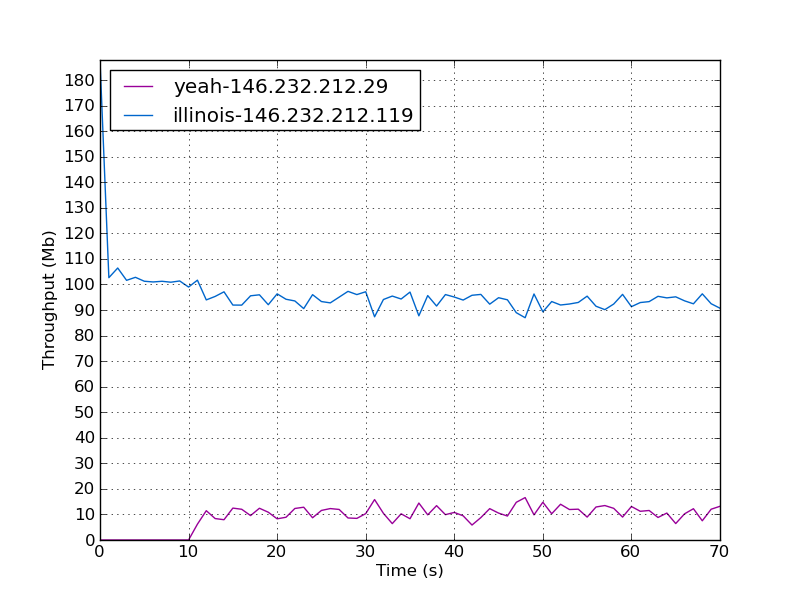
\includegraphics[width=\linewidth]{exp29.png}
	\caption{Illinois commences transmission first, and is joind by YeAH after 10 seconds. Illinois maintains
		a mean throughput of 93 Mbps, while YeAH maintains a very low mean throughput of 10 Mbps.}
	\label{fig:illinois_yeah}
\end{figure}

\begin{figure}[p]
	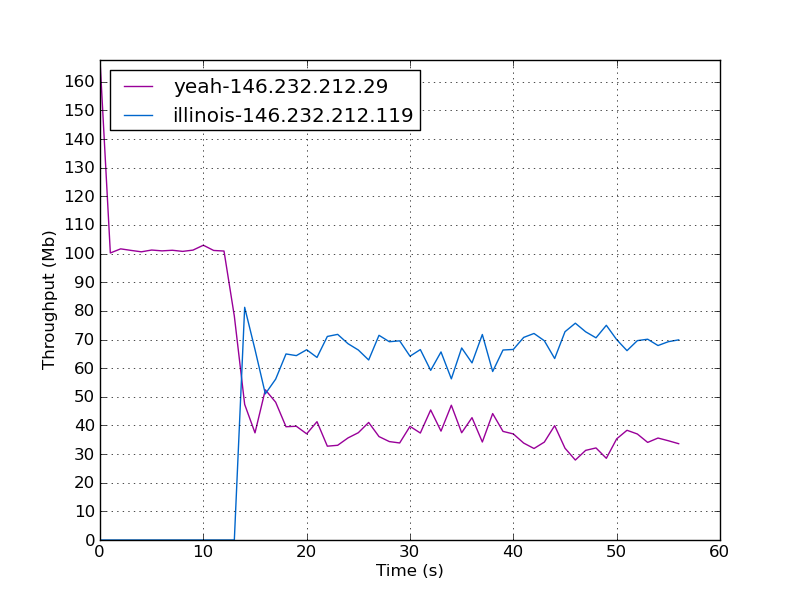
\includegraphics[width=\linewidth]{exp29b.png}
	\caption{YeAH is now allowed to begin transmission before Illinois. Although still less than Illinois,
		YeAH now maintains a much higher than before mean throughput of 37 Mbps, whilst Illinois has
		a lower than before mean throughput of 67 Mbps.}
	\label{fig:yeah_illinois}
\end{figure}

\subsection{LP}
\label{subsec:lp}
From table \ref{table:lp} it is clear that LP is able to co-exist with itself, Hybla, Reno, YeAH, and Cubic.
Just as with Hybla in section \ref{subsec:hybla}, LP fares badly against Illinois, BIC, Westwood, and Scalable.

\begin{table}[h!]
	\begin{center}
		\begin{tabular}{| c | c | l |}
    			\hline
			\multicolumn{3}{|c|}{Mean Throughput (Mbps)} \\
    			\hline
    			LP &  \multicolumn{2}{|c|}{Other}  \\
			\hline
    			38 & 65 & HTCP \\
			\hline
    			54 & 48 & Hybla \\
			\hline
    			33 & 70 & Illinois \\
			\hline
    			53 & 50 & LP \\
			\hline
    			95 & 10 & Vegas \\
			\hline
    			50 & 53 & Reno \\
			\hline
    			29 & 74 & BIC \\
			\hline
    			13 & 90 & Westwood \\
			\hline
    			50 & 53 & YeAH \\
			\hline
    			55 & 47 & Cubic \\
			\hline
    			42 & 61 & Highspeed \\
			\hline
    			27 & 76 & Scalable \\
    			\hline
    		\end{tabular}
  	\end{center}
  	\caption{Mean throughput of LP against other TCP variants.}
	\label{table:lp}
\end{table}

\subsection{Vegas}
\label{subsec:vegas}
TCP Vegas is able to co-exist with itself. Each Vegas client has a mean throughput of about 50 Mbps. Vegas performs very poorly against
all other TCP variants, achieving a mean throughput of anything between 8 and 13 Mbps, depending on which TCP variant it competes against.
This is demonstrated by figure \ref{vegas_reno}.


\begin{figure}[p]
	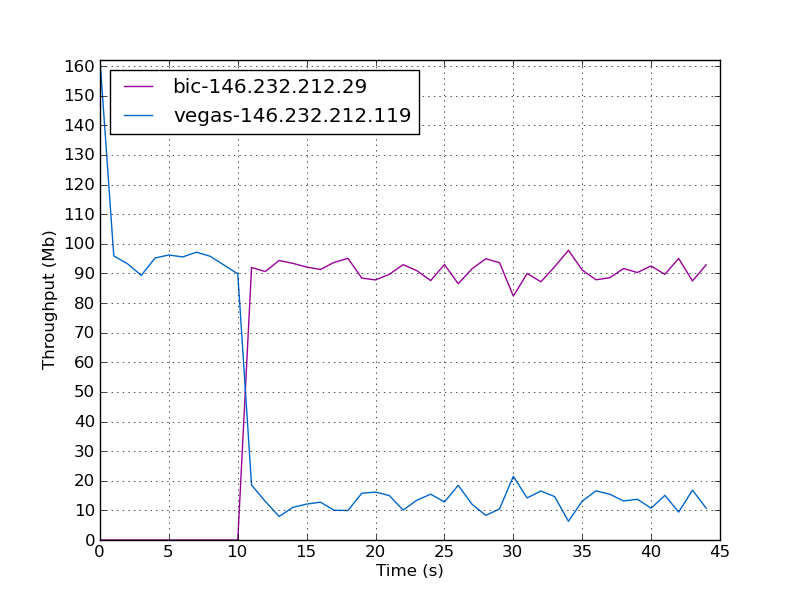
\includegraphics[width=\linewidth]{exp44.png}
	\caption{Vegas begins transmission, followed by BIC ten seconds later. BIC immediately achieves a mean throughput of
		91 Mbps, while Vegas is reduced to a mean throughput of 13 Mbps.}
	\label{fig:vegas_reno}
\end{figure}

\subsection{Scalable}
\label{subsec:scalable}

\section{Technical Difficulties}
\label{sec:diff}

\section{Future Improvements}
\label{sec:imp}

\section{Conclusion}
\label{sec:conc}


\hbadness=5000
\vbadness=5000
\bibliographystyle{plain}
\bibliography{sample}

\end{document}

%===============================================================================
% End of sample.tex
%===============================================================================

